
% XELATEX
% !TEX TS-program = xelatex

%% Based on a TeXnicCenter-Template by Gyorgy SZEIDL.
%%%%%%%%%%%%%%%%%%%%%%%%%%%%%%%%%%%%%%%%%%%%%%%%%%%%%%%%%%%%%

%------------------------------------------------------------
%
\documentclass[a4paper,12pt]{report}%%
%Options -- Point size:  10pt (default), 11pt, 12pt
%        -- Paper size:  letterpaper (default), a4paper, a5paper, b5paper
%                        legalpaper, executivepaper
%        -- Orientation  (portrait is the default)
%                        landscape
%        -- Print size:  oneside (default), twoside
%        -- Quality      final(default), draft
%        -- Title page   notitlepage, titlepage(default)
%        -- Columns      onecolumn(default), twocolumn
%        -- Equation numbering (equation numbers on the right is the default)
%                        leqno
%        -- Displayed equations (centered is the default)
%                        fleqn (equations start at the same distance from the right side)
%        -- Open bibliography style (closed is the default)
%                        openbib
% For instance the command
%           \documentclass[a4paper,12pt,leqno]{article}
% ensures that the paper size is a4, the fonts are typeset at the size 12p
% and the equation numbers are on the left side
%






\usepackage{fontspec}
%\usepackage{amsmath}%
\usepackage{amsfonts}%
\usepackage{amssymb}%
\usepackage{graphicx}
%-------------------------------------------
\newtheorem{theorem}{Theorem}
\newtheorem{acknowledgement}[theorem]{Acknowledgement}
\newtheorem{algorithm}[theorem]{Algorithm}
\newtheorem{axiom}[theorem]{Axiom}
\newtheorem{case}[theorem]{Case}
\newtheorem{claim}[theorem]{Claim}
\newtheorem{conclusion}[theorem]{Conclusion}
\newtheorem{condition}[theorem]{Condition}
\newtheorem{conjecture}[theorem]{Conjecture}
\newtheorem{corollary}[theorem]{Corollary}
\newtheorem{criterion}[theorem]{Criterion}
\newtheorem{definition}[theorem]{Definition}
\newtheorem{example}[theorem]{Example}
\newtheorem{exercise}[theorem]{Exercise}
\newtheorem{lemma}[theorem]{Lemma}
\newtheorem{notation}[theorem]{Notation}
\newtheorem{problem}[theorem]{Problem}
\newtheorem{proposition}[theorem]{Proposition}
\newtheorem{remark}[theorem]{Remark}
\newtheorem{solution}[theorem]{Solution}
\newtheorem{summary}[theorem]{Summary}
\newenvironment{proof}[1][Proof]{\textbf{#1.} }{\ \rule{0.5em}{0.5em}}

%------------All done to create a subsubsubsection command with numbering-----------
\usepackage[T1]{fontenc}
%\usepackage[latin1]{inputenc}
\usepackage[a4paper]{geometry}
\usepackage{lmodern}
\usepackage[english]{babel}
\usepackage{hyperref}
\hypersetup{
  colorlinks,
  citecolor=blue,
  filecolor=blue,
  linkcolor=blue,
  urlcolor=blue}
\setcounter{secnumdepth}{3}
% -------------------------------------------------------------
\setcounter{tocdepth}{2} %depth of table of contents
% \setcounter{secnumdepth}{-1}


\usepackage{setspace}
\usepackage{pslatex,palatino,avant,graphicx,color}
\usepackage{titlesec}
\titleformat{\chapter}[display]
{\normalfont\huge\bfseries\centering}{\thechapter}{20pt}{\Huge}
\newcommand{\cchapter}{\chapter}
\titleformat{\cchapter}[display]
{\normalfont\tiny\bfseries\centering}{\thecchapter}{12pt}{\tiny}
\usepackage{appendix}
\usepackage{float}

\usepackage[utf8x]{inputenc}
%\usepackage[utf8]{inputenc}
\usepackage[numbers,sort&compress]{natbib}
\usepackage{geometry}
\usepackage{subcaption}

\usepackage{fourier}
\DeclareMathAlphabet{\mathcal}{OT1}{pzc}{m}{it}
\DeclareSymbolFont{letters}{OML}{cmm}{m}{it}
\usepackage{mathtools}
%\DeclarePairedDelimiter{\ceil}{\lceil}{\rceil}
\usepackage{amsfonts, amssymb, bm}
\usepackage{booktabs}  % for \toprule ...
\usepackage{caption}
\usepackage{verbatim}
\usepackage{enumitem}
\newcommand{\dd}[1]{\mathrm{d}#1}

\usepackage{graphicx, type1cm, lettrine}
\usepackage{qtree}
\usepackage[dvipsnames, table]{xcolor}
\usepackage{collcell}
\usepackage{pgf}
\usepackage{forest}
\usepackage{setspace}
\usepackage{pgfplots}
\usepackage{tikz}
\usetikzlibrary{shapes.geometric}
\usetikzlibrary{arrows.meta,arrows}
\usepackage{bidipoem}
\usepackage{polyglossia} % <3
\setmainlanguage{english}
\setotherlanguage{arabic}
\newfontfamily\arabicfont  [Script=Arabic, Scale=1.5]{Scheherazade}
\usepackage[numbers,sort&compress]{natbib}
\usepackage{float}
\usepackage{footnote}


\begin{document}
\thispagestyle{empty}
\begin{centering}
\large{\textbf{\\[1cm]{Learning Meters of Arabic Poems with \\ Deep Learning}}}\\[5cm]
\normalsize{}
A Thesis Presented to the Faculty\\
 of\\
 Nile University\\[5cm]
In Partial Fulfillment\\
of the Requirements for the Degree\\
of Master of SCIENCE\\[3cm]
By\\
Moustafa Alaa Mohamed\\
July 2018\\
\end{centering}
\normalsize{}



\newpage 
\thispagestyle{empty}
\begin{centering}
\normalsize{}
CERTIFICATION OF APPROVAL\\[3cm]
Learning Meters of Arabic Poems with \\ Deep Learning\\[4cm]
 By\\
Moustafa Alaa Mohamed\\[4cm]
\end{centering}

\hspace{-1.7em}
\rule[0em]{19em}{0.5pt} \hspace{4em} \rule[0em]{11em}{0.5pt} \\
\hspace{1em}
Dr. Samhaa El-Beltagy	(Chair)	\hspace{9.4em} Date\\
Professor of Electrical and Computer Engineering \\[1cm]
\hspace{1em}
\rule[0em]{19em}{0.5pt} \hspace{4em} \rule[0em]{11em}{0.5pt} \\
\hspace{1em}
Dr. Waleed Yousef \hspace{14.8em}  Date\\
Professor of Computer Science \\[1cm]
\hspace{1em}

\normalsize{}
\newpage 
\pagenumbering{roman} 

\renewcommand{\contentsname}{\uppercase{Table of Contents}}


\newpage


\addcontentsline{toc}{chapter}{Dedication}
%\cchapter*{\textit{\LARGE{\mdseries{Dedication}}}}

%\textit{\\To all my family members, especially my mum and dad, to my predestined and future life mate to be by gods will, and to all my lovely friends, who supported me and have always stood by my side through all times.}

\newpage
\addcontentsline{toc}{chapter}{Acknowledgment}
\cchapter*{\LARGE{\mdseries{\uppercase{Acknowledgment}}}}
%I would like to acknowledge and express my heartfelt gratitude to the persons who have made the achievement of my Master of Science degree possible: \\\\
%Dr. Ahmed Samir Fahmy, for his outstanding assistance and guidance, encouragement, and support all the way.\\\\
%Dr. Ahmed El-Antably, Dr. Nermin Fawzy, and Dr. Mustafa Hunter for their great share and effort in this research.\\\\
%All the Nile University Faculty Members and Staff. \\\\
%Most especially to my family for their help and patience.\\\\
%And above all to God, who have made all things possible.



\newpage
\addcontentsline{toc}{chapter}{Table of Contents}
\tableofcontents
\newpage
\addcontentsline{toc}{chapter}{List of Figures} 
\renewcommand\listfigurename{\uppercase{List of Figures}}
\listoffigures 
\newpage
\addcontentsline{toc}{chapter}{List of Tables}
\renewcommand\listtablename{\uppercase{List of Tables}}
\listoftables 

%\renewcommand\refname{your title for Bib.}
%\renewcommand\abstractname{your title for abstract}

\newpage

\pagenumbering{arabic}
%%%NOTE: Abstract is not attractive need to be revised
\newpage


\addcontentsline{toc}{chapter}{Thesis Outline}
\begin{spacing}{1}\cchapter*{\LARGE{\mdseries{Thesis Outline}}}\end{spacing}
The coming chapters are arranged as follows:
\begin{itemize}
\item Chapter 1: Presents some basic introduction and background knowledge as regards the Arabic Poem and its definitions. Also, it contains details about the Arabic language and some feature used during our work.
  \item Chapter 2: Background related to Al-Arud science and Deep Learning fundamentals. 
  \item Chapter 3: Literature Review for the previous work in this topic.    
  \item Chapter 4: Introduces the essential pre-processing steps, and the justification for their need. Pre-processing steps are data extraction, data cleansing and data format.
  \item Chapter 5: introduces the data encoding techniques used and the effect of each one. Also, it contains some comparisons between the three techniques used.
  \item Chapter 6: presents the model's details and how we chose the model and the architecture and hyper-parameters details.
  \item Chapter 7: Results and discussion.
  \item Chapter 8: Conclusion and future work
\end{itemize}


 \newpage



\addcontentsline{toc}{chapter}{Abstract}

\begin{spacing}{1}\cchapter*{\LARGE{\mdseries{ABSTRACT}}}\end{spacing}


People can easily determine whether a piece of writing is a poem or prose, but only specialists can determine the class of poem.

In this thesis, We built a model that can classify poems according to their meters; a forward step towards machine understanding of Arabic language.

A number of different deep learning models are proposed for poem meter classification. As poems are sequence data, then recurrent neural networks are suitable for the task. We have trained three variants of them, LSTM, GRU with different architectures and hyper-parameters. Because meters are a sequence of characters, then we have encoded the input text at the character-level, so that we preserve the information provided by the letters succession directly fed to then models. Besides, We introduce a comparative study on the difference between binary and one-hot encoding regarding their effect on the learning curve. We also introduce a new encoding technique called \textit{Two-Hot} which merges the advantages of both \textit{Binary} and \textit{One-Hot} techniques.


Artificial Intelligence currently works to do the human tasks such as our problem here. Our target in this thesis is to achieve the human accuracy which will make it easy for anyone to know the meter for any poem without referring to the language experts or to study the whole field to achieve it.

In this thesis, We will explain how to use the deep learning to classify the Arabic poem to classes. Also, explain in details the feature of Arabic poem and how to deal with this features. Besides, We explain how can anyone work with Arabic text encoding with a dynamic way to encode the text at the character level and deal with the Arabic text feature example the  \textit{Tashkeel}.

%\end{abstract}
%qualitative

\newpage

%%%NOTE: Introduction is too long and include a lot of background details it should be small and need to move the details into background
\chapter{\uppercase{Introduction}}


%\begin{spacing}{1.5}\section*{\LARGE{\mdseries{Thesis Outline}}}

 

  Arabic is the fifth most widely spoken language\footnote{\textit{according to the 20th edition of Ethnologue, 2017}}. It is written from right to left. Its
alphabet consists of 28 primary letters, and there are 8 more derived letters
from the basic ones, so the total count of Arabic characters is 36 characters.
The writing system is cursive; hence, most letters join to the letter that comes
after them, a few letters remain disjoint.

\section{Arabic Poetry } %%
%% Introduction; the circumstances before alarud
Arabic poetry(\textarabic{الشعر العربى}) is the earliest form of Arabic literature. It dates back to the Sixth century. Poets have written poems without knowing exactly what rules which make a collection of words a poem. People recognize poetry by nature, but only talented ones can write poems. This was the case until \textit{Al-Farahidi} (718 – 786 CE) has analyzed the
Arabic poetry, then he came up with that the succession of consonants and vowels
produce patterns or \textit{meters}, which make the music of poetry.  He has
counted them fifteen meters.  After that, a student of \textit{Al-Farahidi} has
added one more meter to make them sixteen. Arabs call meters \textarabic{بحور}
which means ``\textit{seas}''. The study of Arabic Poems classification is named \textbf{Al-Arud (\textarabic{العَروض})}. It takes too much time for anyone to be an expert in this field. 
\section{Deep Learning}

Deep Learning also named Deep Neural Network is part of Machine Learning algorithms. Deep Learning is trying to simulate the human brain into Neural dependency.  Using Deep Learning, we can achieve better learning results from the data. Deep Neural Network needs a huge amount of data to achieve the expected learning curve and results. It also needs a massive amount of computation to build the networks which are based on an artificial neural network. We used the Recurrent Neural Network (RNN) to work on the Arabic Text which shown its ability to achieve outstanding performance over the text problem data. We also used LSTM to solve the long dependency issue in RNN. We will go deep into the Background section (add deep learning section reference).

\section{Thesis Objectives}
In this study, we work to classify the poem and utilize the latest technologies check the class of poem. We also worked to achieve near human expert results which make our work is a breakthrough in the field concerning the results compared to the current achieved results. Figure \ref{fig:thesis_cycle} shows the steps.,
\begin{figure}[h!]
  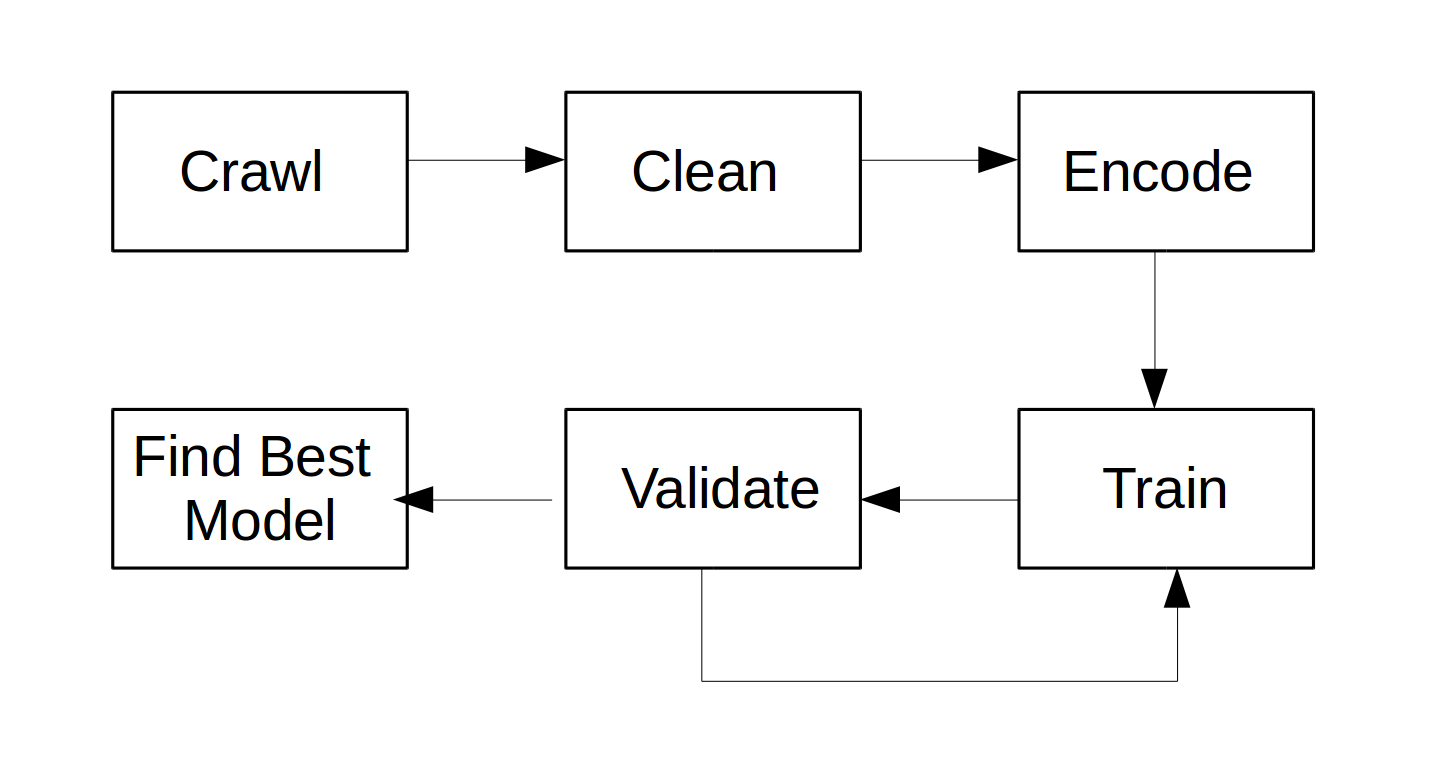
\includegraphics[width=\linewidth,height=6cm]{./Figures/Master_Cycle.png}
  \caption{Thesis Working Steps.}
  \label{fig:thesis_cycle}
\end{figure}

\begin{itemize}
\item Crawling the data from the available sources with labeling.
\item Clean and transform the data.
\item Encode the data into a way to be input to the model to work on it. We used many encoding methods and compared each of them.
\item Train the RNN model into the cleaned data.
\item Validate and test the model.
\item Enhance the model.

\end{itemize}








%\begin{figure}
%	
%	

\begin{tikzpicture}[scale=0.9]
\begin{axis}[
    symbolic x coords={Taweel,
   Kamel,
   Baseet,
   Khafeef,
   Wafeer,
   Rigz,
   Raml,
   Motakarib,
   Sar'e,
   Monsafeh,
   Mogtath,
   Madeed,
   Hazg,
   Motadarik,
   Moktadib,
   Modar'e
    },
    xtick=data,
    % the following x label positioning does work here.
    every axis y label/.style= {at={( 0.1, 1.1)}, anchor=north},
    %ylabel style={font=\footnotesize},
    xticklabel style = {font=\footnotesize},
    ylabel={Class size},
    x=0.4cm,
    x tick label style={rotate=60, anchor=east}, 
    % Y ticks configurations
    y tick label style={/pgf/number format/.cd,%
      scaled y ticks = false,
      set thousands separator={,},
      fixed},]
    \addplot[ybar,fill=myBlue] coordinates {
        (Taweel, 416428)
        (Kamel,  370116)
        (Baseet, 244583)
        (Khafeef,     157880)
        (Wafeer,     143148)
        (Rigz,     119286)
        (Raml,     79560)
        (Motakarib,     63613)
        (Sar'e,     59370)
        (Monsafeh,     28768)
        (Mogtath,     18062)
        (Madeed,     7808)
        (Hazg,     7468)
        (Motadarik,     5144)
        (Moktadib,     799 )
        (Modar'e,     288 )
    };
\end{axis}
\end{tikzpicture}

%	
%	\caption{Meter names are on the $x$-axis, size  is on the $y$-axis.}
%	\label{data_size}
%\end{figure}




\newpage

\chapter{\uppercase{Background}}
Each Arabic letter represents a consonant, which means that short vowels are not
represented by the 36 characters, for this reason, the need of \textit{diacritics}
rises. \textit{Diacritics} are symbols that comes after a letter to state the
short vowel accompanied by that letter. There are four diacritics \textarabic{◌َ} \textarabic{◌ُ}
\textarabic{◌ِ} \textarabic{◌ْ} which represent the following short vowels
/\textit{a}/, /\textit{u}/, /\textit{i}/ and \textit{no-vowel} respectively,
their names are \textit{fat-ha, dam-ma, kas-ra and sukun} respectively.  The first
three symbols are called \textit{harakat}. Table \ref{tables:diacritics_dal}
shows the 4 diacritics on a letter.



% table: dal with diacritics
\begin{table}[H]
	\centering
	\begin{tabular}{c c c c c c}
		%\hline
		\toprule
		\textbf{\small{Diacritics}}     & \small{\textit{without}} & \small{\textit{fat-ha}} &
		\small{\textit{kas-ra}} & \small{\textit{dam-ma}} & \small{\textit{sukun}}\\
		%\hline
		\midrule
		\textbf{\small{Shape}}   & \textarabic{د} & \textarabic{دَ} & \textarabic{دِ} &
		\textarabic{دُ} & \textarabic{دْ}\\
		%\hline
		\bottomrule
	\end{tabular}
	\caption{\textit{Diacritics on the letter  \textarabic{ د }}}\label{tables:diacritics_dal}
\end{table}



There are two more sub-diacritics made up of the basic four to represent two
cases:
\begin{definition}\label{def:shadaa_definition}
  \textbf{Shadaa}  \hfill \\
to indicate the letter is doubled. Any letter with
shaddah (\textarabic{ ّ } ) the letter should be duplicated: first letter with a
constant (sukoon) and second letter with a vowel (haraka) \cite{Alnagdawi2013}; Table  \ref{tables:shadda_dal}
shows the dal with shadda and the original letters.
% table: dal with shadda

\begin{table}[H]
	\centering
	\begin{tabular}{c c c}
		%\hline
		\toprule
		\textbf{\small{Diacritics}} & \small{\textit{letter with Shadda }} & \small{\textit{letters without shadaa  }} \\
		%\hline
		\midrule
		\textbf{\small{Shape}}  & \textarabic{دَّ} &  \textarabic{دْدَ}\\
		%\hline
		\bottomrule
	\end{tabular}
	\caption{\textit{Shadaa diacritics on the letter  \textarabic{ د }}}\label{tables:shadda_dal}
\end{table}

\end{definition}

\begin{definition}\label{def:tanween_definition}
  \textbf{Tanween} \hfill \\
  %%% \ref{defa} and \ref{defb}
  is doubling the short vowel, and can convert
Tanween fathah, Tanween dhammah or Tanween kasrah by
replacing it with the appropriate vowel ( ُ◌ – dhammah, َ◌ –
fathah or ِ◌ –kasrah ) then add the Noon letter with constant to the end of the word \cite{Alnagdawi2013}. Table \ref{tables:Tanween_dal}
shows the difference between the original letter and the letter with Tanween

\begin{table}[H]
	\centering
	\begin{tabular}{c c c}
		%\hline
		\toprule
		\textbf{\small{Diacritics}} & \small{\textit{letter with tanween }} & \small{\textit{letters without tanween}} \\
		%\hline
		\midrule
          
          \textbf{\small{Tanween Fat-ha}}  & \textarabic{دً} &  \textarabic{دَ+نْ}\\
          \textbf{\small{Tanween Dam-ma}}  & \textarabic{دٌ} &  \textarabic{دُ+نْ}\\
          \textbf{\small{Tanween Kas-ra}}  & \textarabic{دٍ} &  \textarabic{دِ+نْ}\\
          
	
		\bottomrule
	\end{tabular}
	\caption{\textit{Tanween diacritics on the letter  \textarabic{ د }}} \label{tables:Tanween_dal}
\end{table}


\end{definition}

 Arabs pronounce the sound \textit{/n/} accompanied \textit{sukun} at the end the indefinite words, that sound corresponds to this
letter \textarabic{نْ}, it is called \textit{noon-sakinah}, however, it is
just a phone, it is not a part of the indefinite word, if a word comes as a
definite word, no additional sound is added. Since it is not an essential sound,
it is not written as a letter, but it is written as  \textit{tanween}
\textarabic{◌ٌ ◌ً ◌ٍ}.
% adding tanween and its relationship to the previous letter
\textit{Tanween} states the sound \textit{noon-sakinah}, but as you have noticed,
there are 3 \textit{tanween} symbols, this because  \textit{tanween} is added as
a diacritic over the last letter of the indefinite word, one of the 3 harakat\textit{harakat} accompanies the last letter, the last letter's \textit{harakah}
needs to be stated in addition to the sound \textit{noon-sakinah}, so
\textit{tanween} is doubling the last letter's \textit{haraka}, this way the last
letter's \textit{haraka} is preserved in addition to stating the sound
\textit{noon-sakinah}; for example, \textarabic{رَجُلُ + نْ} is written
\textarabic{رَجُلٌ} and  \textarabic{رَجُلِ + نْ} is written \textarabic{رَجُلٍ}. 


Those two definition, Definition ~\ref{def:shadaa_definition} and Definition ~\ref{def:tanween_definition}  will help us to reduce the dimension of the letter's feature vector as we will see in \textit{preparing data} section.


Diacritics makes short vowels clearer, but they are not necessary.
Moreover, a phrase without full diacritics or with just some on some letters is
right linguistically, so it is allowed to drop them from the text.

% Diacritics in Unicode
In Unicode, Arabic diacritics are standalone symbols, each of them has its own
unicode. This is in contrast to the Latin diacritics; e.g., in the set
\textit{\{ê, é, è, ë, ē, ĕ, ě\}}, each combination of the letter \textit{e} and a diacritic is represented by one unicode.

\newpage

\section{Arabic Arud Science}
reference is the book .... to be added
\begin{definition}\label{def:arud}
  \textbf{Arud} \hfill \\
In Arabic Arud natively has many meanings (the way, the direction, the light clouds and Mecca and Madinah\footnote{\textit{Mecca and Madinah are two cities in  Saudi Arabia}.}. Arud is the science which studies The Arabic Poem meters and the rules which confirm if the Poem is sound meters \& broken meters. It named Arud because some people said he put this science in Arud place \textarabic{العَروض} \textit{with fat-ha, not with dam-ma such as the science name \textarabic{العُروض} } between Mecca and Madinah.
\end{definition}

The Author of this science is \textit{Al-Farahidi} (718 – 786 CE) has analyzed the
Arabic poetry; then he came up with that the succession of consonants and vowels
produce patterns or \textit{meters}, which make the music of poetry. He was one of the famous people who know The melodies and the musical parts of speech. He has
counted them fifteen meters.  After that, a student of \textit{Al-Farahidi} has
added one more meter to make them sixteen. Arabs call meters \textarabic{بحور}
which means "\textit{seas}." Poets have written poems without knowing exactly what rules which make a collection of words a poem.

The Reasons which makes \textit{Al-Farahidi} put this science is

  \begin{itemize}
  \item Protect the Arabic Poems from the broken meters.
  \item Distinguish between the original Arabic Poem and the non-poem or from the prose.
    \item Make the rules clear and easy for anyone who needs to write a poem.
  \end{itemize}
  
    Some people said that the one-day Al-Farahidi was walking into the metal-market and he was said some of the poems and for some reasons the knock of the metals matched the musical sound of the poem he was saying then he got an idea to explore the Arud of the poems.
\newpage
    \subsection{Feet Representation}
    A meter is an ordered sequence of feet. Feet are the basic
units of meters; there are ten of them.
\begin{definition}\label{def:feet}
  \textbf{Feet} \hfill \\  A Foot consists of
a sequence of \textbf{Sukun} (Consonants) represented as (0) and \textbf{Harakah} (Vowels) (/). Traditionally, feet are represented by mnemonic words called tafa’il \textarabic{تفاعيل}.
\end{definition}

Feets consists of three parts (Reasons \textarabic{أسباب}, Wedge \textarabic{وتد}, Breaks \textarabic{فواصل}).
\begin{itemize}
\item \textbf{Reasons (\textarabic{أسباب})}: It has two types
  \begin{enumerate}
  \item \textbf{Light (\textarabic{سبب خفيف})} which happens when we have the first letter is harakah and the second is sukun (/0) example (\textarabic{هَبْ, لَمْ}).
    \item \textbf{Heavy (\textarabic{سبب ثقيل})} which happens when we have two harakah letter (//) example (\textarabic{لَكَ, بِكَ}).
    \end{enumerate}
    \item \textbf{Wedge (\textarabic{وتد})}: It has two types
  \begin{enumerate}
  \item \textbf{Combined Wedge (\textarabic{وتد مجموع})} which happens when we have two harakah letters followed by sukun (//0) example (\textarabic{مَشَى, عَلَى}).
    \item \textbf{Separated Wedge (\textarabic{وتد مفروق})} which happens when we have two harakah and in between a sukun letter (/0/) example (\textarabic{مُنْذُ, مِصْرُ}).
    \end{enumerate}
    \item \textbf{Breaks (\textarabic{فواصل}}): It has two types
  \begin{enumerate}
  \item \textbf{Small Break (\textarabic{فاصلة صغرى}}) which happens when we have three harakah letters followed by a sukun letter (///0) example (\textarabic{ذَهَبُوا, سُفُناً}).
    \item \textbf{Big Break (\textarabic{فاصلة كبرى}}) which happens when we have four harakah letters followed by a sukun letter  (////0) example (\textarabic{جَعَلَهُمْ}).\footnote{\textit{Some of Arab linguistic scientist assume the small Breaks as a combination between big reason and small reason. Same for the Big Breaks assumed to be a combination between Big reason and Combined Wedge. So, they didn't assume we have three types of feet it is only pure two and any other feets constructed from this two. In this thesis we assume there are three feets }.}
    \end{enumerate}
  \end{itemize}
  
\newpage
  \subsubsection{Rules for Arabic Letters Representation}
  Arabic letter has one general rule in the poem representation which is we represent only the letters which is (spoken) not the written which means the letters with phonatics not the written. We have give the below rules as a results of the general rule.

  \begin{itemize}
  \item Any letter with \textit{harakah} represented as (/).
  \item Any letter with \textit{sukun} represented as (0).
  \item Any letter with shaddah represented by two letters the first one will be \textit{sukun} and the second letter will be \textit{harakah} represented as (0/) example (\textarabic{مُحَمََّد}) will be (//0//0).
  \item Any letter with tanween represented by two letters the first one is \textit{haraka} (/) and the second is \textit{sukun}.
  \item Alef without hamze (\textarabic{همزة الوصل}) and Wow Algmaa are not represented example (\textarabic{وُاعلَموا}) will be (/0//0)
  \item If we have a letter which is not written but (spoken) so, we will represent it example (\textarabic{هذا}) it include Alef but not written (\textarabic{هاذا}) the representation will be (/0/0).
  \item If we have \textit{Meem Aljamaa} with harakah so, it represented with \textit{Mad} example (\textarabic{هُمُ}) will be (//0) .
  \item \textit{Alef Mad} (\textarabic{آ}) will be two letters \textit{Alef with harakah} and \textit{Alef with sukun} example (\textarabic{آدَمُ}) will be (/0//).
    \item if the verse ended with \textit{harkah} we will add \textit{sukun} to it.
    
    
    \end{itemize}
Exampel: (note: the below representation is not complete )
\begin{Arabic}
	\begin{traditionalpoem*}
وَجَدتُ الناسَ مَيتاً مِثلَ حَيٍّ *** بِحُسنِ الذِكرِ أَو حَيّاً كَمَيتِ
وَجَدْتُنْنَاْ سَمَيْتَنْمِثْ لَحَيْيِنْ *** بِحُسْنِذْذِكْ رِأَوْحَيْيَنْ كَمَيْتِيْ

	\end{traditionalpoem*}
\end{Arabic}
    
\newpage

\subsection{Arabic Poetry Feets}

Arabic poetry feets has ten tafa'il \textarabic{تفاعيل} (scansion)  any peom constructed from these feets. They are eight from writing (syntax) prespective, But it ten in the rules.
\begin{savenotes}

\begin{table}[H]
  \centering
  \begin{tabular}{|c|c|c|c|}
    \hline
    \textbf{\#} & \textbf{Feet} & \textbf{Scansion} & \textbf{Construction} \\
    \hline
    1 & \textarabic{فَعُولُنْ}  & \texttt{0/0//} & combined wedge (\textarabic{فعو}) and small reason (\textarabic{لن})   \\
    2 &\textarabic{مَفاعِيلُنْ}& \texttt{0/0/0//} & combined wedge (\textarabic{مفا}) and two light reasons (\textarabic{عي}) (\textarabic{لن})   \\
    3 &\textarabic{مُفَاعَلَتُنْ}& \texttt{0///0//}  &    combined wedge (\textarabic{مفا}), heavy reason (\textarabic{عل}) and light reason (\textarabic{تن}) \\
    4 &\textarabic{فَاعِلاَتُنْ} & \texttt{0/0//0/}   & light reason (\textarabic{فا}), combined wedge (\textarabic{علا}) and light reason (\textarabic{تن})   \\
    5 &\textarabic{فَاعِ لاتُنْ} & \texttt{0/0//0/}  &  Separated wedge (\textarabic{فاع}) and two light reason (\textarabic{لا})(\textarabic{تن}) \footnote{\textit{We separated the letters (\textarabic{ع}) and (\textarabic{لا}) in (\textarabic{فاع لاتن}) to show that this part is separated wedge and distinguish between this feet  and (\textarabic{فاع لاتن}) which contains combined wedge  }.}  \\    
    6 &\textarabic{فَاعِلُنْ}  & \texttt{0//0/}   & light reason (\textarabic{فا}) and combined wedge (\textarabic{علن})\\
    7 &\textarabic{مُتَفَاعِلُنْ}& \texttt{0//0///}  & heavy reason (\textarabic{مت}), light reason (\textarabic{فا}) and combined wedge (\textarabic{علن})  \\
    8 &\textarabic{مَفْعُولاَت} & \texttt{0//0///}   & two light reason (\textarabic{مف})(\textarabic{عو}) and separated wedge (\textarabic{لات}) \\
    9 &\textarabic{مُسْتَفْعِلُنْ} & \texttt{0//0/0/}  &  two light reason (\textarabic{مس})(\textarabic{تف}) and combination wedge (\textarabic{علن}) \\
    10 &\textarabic{مُسْتَفْعِ لُنْ} & \texttt{0//0/0/}  & light reason (\textarabic{مس}), separated wedge  (\textarabic{تفع}) and light reason  (\textarabic{لن})\footnote{\textit{We separated the letters (\textarabic{ع}) and (\textarabic{ل}) in (\textarabic{مستفع لن}) to show that it ends with a separated wedge and distinguish between this feet  and (\textarabic{مستفعلن}) which contains combined wedge }}\\
    
    
    \hline
  \end{tabular}
  \caption{The ten feet of the Arabic meters. }\label{arud:feet}
\end{table}
    \end{savenotes}

%% Every digit (\texttt{/} or \texttt{0}) represents
%%    the corresponding diacritic over a letter in the feet. \texttt{/} corresponds to
%%    a\textit{harakah} ( \textarabic{◌َ}, \textarabic{◌ُ}, or \textarabic{◌ِ}) and \texttt{0}
%%    corresponds to a \textit{sukun} (\textarabic{◌ْ}). Any \textit{mad} (\textarabic{و, ا, ى}) is
%%    equivalent to \texttt{0}, \textit{tanween} is equivalent to \texttt{0/}, and \textit{shaddah} is
%%    equivalent to \texttt{/0}%

    \newpage
\begin{definition}\label{def:meter}
  \textbf{Meter} \hfill \\
  %%%% What is rtythm,feet
  Poetic meters define the basic rhythm of the poem. Each meter is described by a set of ordered feet which can
be represented as ordered sets of consonants and vowels \cite{Almuhareb2015}.

% \textbf{Some conventions and terminologies}:

% What are poems and terminologies?
% What does a poem look like? bayt, shatr, ....
\begin{Arabic}
	\begin{traditionalpoem*}
          ولد الهدى فالكائنات ضياء *** وفم الزمان تبسم وثناء انشاء
          الروح والملأ الملائك حوله *** للدين والدنيا به بشراء

	\end{traditionalpoem*}
\end{Arabic}%



\end{definition}


\begin{definition}\label{def:verse}
  \textbf{Arabic Verse} \hfill \\ refers to "poetry" as contrasted to prose. Where the common unit of a verse is based on meter or rhyme, the common unit of prose is purely grammatical, such as a sentence or paragraph \footnote{\textit{ https://en.wikipedia.org/wiki/Verse\_(poetry)}.}. A verse know as \textit{Bayt} in Arabic \textarabic{بيت}

\end{definition}


\begin{definition}\label{def:shatr}
  \textbf{Shatr} \hfill \\  A verse consists of two halves, each of them is called \textit{shatr} and carries the full meter.  We will use the term \textit{shatr} to refer to a verse's half; whether the right or the left half.
\end{definition}



\begin{definition}\label{def:poem}
  \textbf{Poem} \hfill \\
  is a set of verses has the same meter and rhyme.  

\end{definition}

\bigskip
    
\newpage




\newpage

\chapter{\uppercase{LITERATURE REVIEW}}

\newpage


\chapter{\uppercase{Dataset}}

We have scrapped the Arabic dataset from two big poetry websites:
\textarabic{الديوان}\footnote{\textit{aldiwan.net}}, \textarabic{الموسوعة
	الشعرية}\footnote{\textit{poetry.tcaabudhabi.ae}}. Both are merged into one large
dataset. It is important to note that the verses' diacritic states are not
consistent, this means that a verse can carry full, semi diacritics or it can
carry nothing. The total number of verses is  1,862,046 poetic verses; each verse is
labeled by its meter, the poet who wrote it, and the
age which it was written in. There are 22 meters, 3701 poets and 11
ages; and they are Pre-Islamic, Islamic, Umayyad, Mamluk, Abbasid, Ayyubid, Ottoman,
Andalusian, era between Umayyad and Abbasid, Fatimid and modern.  We are only
interested  in the 16 classic meters which are attributed to \textit{Al-Farahidi},
and they are the majority of the dataset with a total number of 1,722,321
% NOTE: change the public rep.
verses\footnote{https://wwww.github.com/tahamagdy}.

\section{Preparing Data}
\subsection{Data Cleaning}

\newpage

\chapter{\uppercase{Data Encoding}}
\subsection{Arabic Poem Encoding}
\subsubsection{One-Hot encoding}
\subsubsection{Binary Encoding}
\subsubsection{Two-Hot encoding}

\newpage

\chapter{\uppercase{Model training}}

\newpage


\chapter{\uppercase{Results And Discussion}}

\newpage

\chapter{\uppercase{Conclusion and Future Work}}
\section{Future Work}

\newpage

\addcontentsline{toc}{chapter}{References}
\makeatletter
\renewcommand{\ps@plain}{%
\renewcommand\@oddhead{\hfil\normalfont\textrm{\thepage}}%
\renewcommand\@evenhead{}%
\renewcommand\@oddfoot{}%
\renewcommand\@evenfoot{}%
}
\makeatother
\pagestyle{myheadings}
\renewcommand\bibname{\uppercase{References}}
\begin{thebibliography}{999}
\bibitem{Alnagdawi2013}
\bibitem{Almuhareb2015}Abdulrahman Almuhareb
\bibitem{Alkafi1994} Al-Khatib Al tabrisi 1994. Al-Kafi in Al-Arud and Al-Quafi. Al-Khangi Press.
 

    
\bibitem{AlQuaed} القواعد العروضية وأحكام القافية العربية , محمد بن فلاح المطيري
\bibitem{Goodfellow-et-al-2016} Deep Learning,
    author={Ian Goodfellow and Yoshua Bengio and Aaron Courville},
    publisher={MIT Press},
    note={\url{http://www.deeplearningbook.org}},
    year={2016}

    \bibitem{Zeiler2014} Zeiler, M. D. and Fergus, R. (2014). Visualizing and understanding convolutional networks. In ECCV’14.

      \bibitem{Cox2958} Cox, D. R. "The Regression Analysis of Binary Sequences." Journal of the Royal Statistical Society. Series B (Methodological) 20, no. 2 (1958): 215-42. http://www.jstor.org/stable/2983890.
\end{thebibliography}

%\newpage
%\begin{subappendices}
%
%\section{Appendix A}\label{A}
%Please refer to Appendix \ref{C}.
%
%\section{Second appendix}\label{B}
%Please refer to Appendix \ref{A}.
%
%\section{Third appendix}\label{C}
%Please refer to Appendix \ref{B}.
%
%\end{subappendices}
\newpage

\newpage



\thispagestyle{empty}
\begin{centering}
\Huge{\textbf{\\[8cm]\uppercase{Appendices}}}\\[1.2cm]
\end{centering}
\normalsize{}

\newpage
\addcontentsline{toc}{chapter}{Appendices}
\addcontentsline{toc}{section}{Appendix A}
\begin{spacing}{2}
\chapter*{\uppercase{Appendix A}} \label{A}
\section*{Phase Correlation Theory}
Let $D_{1}(x,y)$ and $D_{2}(x,y)$ be the dilated images to be registered, the Fourier transform for both $F_{1}(u,v)$ and $F_{2}(u,v)$ is given by:
\[F_{k}(u,v)= \mathcal{F}\{D_{k}(x,y)\}\]
\begin{equation}\label{eq:fourier}
=\int_{y=-\infty}^{y=\infty}\int_{x=-\infty}^{x=\infty}D_{k}(x,y)\exp^{\left(-i2\pi\omega xy\right)}dxdy
\end{equation}
where, $\mathcal{F}$ is the Fourier operator, $K$ denotes image 1 or 2, $\omega$ is the frequency (in hertz), $x$ and $y$ are the spatial domain coordinates, $u$ and $v$ are the frequency domain coordinates of the two images.

Given two images of size $N\times M$ shifted against each other, according to the Fourier shift property, their Fourier becomes:
\begin{equation}\label{eq:fouriershift}
F_{2}(u,v)= F_{1}(u,v)\exp^{\left(-i2\pi\left(\frac{u\Delta x}{M}+\frac{v\Delta y}{N}\right)\right)}
\end{equation}

The Normalized Cross Power Spectrum ($C(u,v)$) is defined as:
\begin{equation}
C(u,v)= \frac{F_{1}(u,v)\cdot F_{2}(u,v)^{*}}{\left|F_{1}(u,v)\cdot F_{2}(u,v)^{*}\right|}
\end{equation}
where `.' denotes the element-wise product, `*' denotes the complex conjugate.  

Using equation \ref{eq:fouriershift}:
\begin{equation}
C(u,v)= \frac{F_{1}(u,v)\cdot F_{1}(u,v)^{*}\exp^{\left(i2\pi\left(\frac{u\Delta x}{M}+\frac{v\Delta y}{N}\right)\right)}}{\left|F_{1}(u,v)\cdot F_{1}(u,v)^{*}\exp^{\left(i2\pi\left(\frac{u\Delta x}{M}+\frac{v\Delta y}{N}\right)\right)}\right|}
\end{equation}

Since the phase term of $F_{1}(u,v)\cdot F_{1}(u,v)^{*}$ is zero, only the magnitude remains, i.e. $F_{1}(u,v)\cdot F_{1}(u,v)^{*}= \left|F_{1}(u,v)\cdot F_{1}(u,v)^{*}\right|$ and since the magnitude of any complex exponential is 1, the equation drops to:
\[
C(u,v)= \frac{\left|F_{1}(u,v)\cdot F_{1}(u,v)^{*}\right|\exp^{\left(i2\pi\left(\frac{u\Delta x}{M}+\frac{v\Delta y}{N}\right)\right)}}{\left|F_{1}(u,v)\cdot F_{1}(u,v)^{*}\right|}
\]
\begin{equation}
= \exp^{\left(i2\pi\left(\frac{u\Delta x}{M}+\frac{v\Delta y}{N}\right)\right)}
\end{equation}
the inverse Fourier transform of which is a delta function, i.e. a single peak.

The Normalized Cross Correlation ($c$) equals:
\begin{equation}
c= \mathcal{F}^{-1}\{C\}= \delta(x+\Delta x, y+ \Delta y)
\end{equation}

The shift in $x$ and $y$ between the two images $(\Delta x, \Delta y)$ takes the location of the maximum peak in $c$, such that:
\begin{equation}
(\Delta x, \Delta y)= \underset{x,y}{\operatorname{argmax}}\{c\}
\end{equation}

%%%%%%%%%%%%%
\newpage
%%\appendix
%%\appendixpage
%%\addappheadtotoc


% \newpage

\end{document}

% Local Variables:
% TeX-engine: xetex
% End:
